\documentclass[../../main.tex]{subfiles}
\begin{document}
\graphicspath{{figures/}{lectures/01_intro_linear/figures/}}
\section{Introduction \& Linear Models}
\begin{frame}[plain]
  \vfill\begin{center}{\Huge \textcolor{blue}{Introduction \& Linear Models}}\end{center}\vfill
\end{frame}
% Title Slide



%--------------------------------------------------
\begin{frame}{Supervised Learning: Definition}
We observe a dataset of input–output pairs:
\[
\mathcal{D} = \{(x_i, y_i)\}_{i=1}^N,
\]
where
\begin{itemize}
    \item $x_i \in \mathbb{R}^p$ is a feature vector,
    \item $y_i$ is the target label (real-valued for regression, categorical for classification).
\end{itemize}

\begin{block}{Goal}
Learn a function $f: \mathbb{R}^p \to \mathcal{Y}$ such that
\[
f(x) \approx y
\]
for both training and unseen examples.
\end{block}
\end{frame}

%--------------------------------------------------
\begin{frame}{Supervised Learning: Examples}
\begin{itemize}
    \item \textbf{Regression:} $y \in \mathbb{R}$  
    Example: predict house prices from square footage.
    \[
    y = f(x) + \varepsilon
    \]
    \item \textbf{Classification:} $y \in \{1,\ldots,K\}$  
    Example: classify emails as spam or not spam.
    \[
    P(y \mid x) \;\; \text{modeled with logistic regression, SVM, neural nets, etc.}
    \]
\end{itemize}
\end{frame}

%--------------------------------------------------
\begin{frame}{Unsupervised Learning: Definition}
We observe only inputs:
\[
\mathcal{D} = \{x_i\}_{i=1}^N, \quad x_i \in \mathbb{R}^p
\]

\begin{block}{Goal}
Discover hidden structure or representation of the data without labels $y_i$.
\end{block}
\end{frame}

%--------------------------------------------------
\begin{frame}{Unsupervised Learning: Examples}
\begin{itemize}
    \item \textbf{Clustering:} Assign samples into groups
    \[
    \text{Find } C(x_i) \in \{1, \ldots, K\}
    \]
    Example: customer segmentation.
    \item \textbf{Dimensionality Reduction:} Map data into lower-dimensional space
    \[
    z_i = W^T x_i, \quad z_i \in \mathbb{R}^k, \; k \ll p
    \]
    Example: PCA, autoencoders.
    \item \textbf{Density Estimation:} Estimate underlying probability distribution $p(x)$.
\end{itemize}
\end{frame}

%--------------------------------------------------
\begin{frame}{Supervised vs. Unsupervised Learning}
\begin{center}
\begin{tabular}{|c|c|}
\hline
\textbf{Supervised} & \textbf{Unsupervised} \\
\hline
Data: $(x,y)$ pairs & Data: $x$ only \\
Predict outputs $y$ & Discover hidden patterns \\
Regression, classification & Clustering, PCA, autoencoders \\
Loss functions (MSE, cross-entropy) & Objectives (reconstruction, likelihood) \\
\hline
\end{tabular}
\end{center}
\end{frame}


%%%%%%%%%%%%%%%%%%%%%%%%%
\begin{frame}{Linear Regression Models}
We have an input vector $X^T = (X_1, X_2, \ldots, X_p)$ and want to predict a real-valued output $Y$.

\[
f(X) = \beta_0 + \sum_{j=1}^p X_j \beta_j
\]

The variables $X_j$ can come from:
\begin{itemize}
    \item Quantitative inputs
    \item Transformations of inputs (log, $\sqrt{\cdot}$, square, etc.)
    \item Basis expansions, e.g. $X_2 = X_1^2, \; X_3 = X_1^3$
    \item Dummy coding of qualitative inputs
    \item Interactions, e.g. $X_3 = X_1 \cdot X_2$
\end{itemize}
\end{frame}

%-----------------------------------------------

\begin{frame}{Least Squares Estimation}
Given training data $(x_1,y_1), \ldots, (x_N,y_N)$, the least squares method minimizes:

\[
\text{RSS}(\beta) = (y - X\beta)^T (y - X\beta)
\]

where $X$ is the $N \times (p+1)$ design matrix and $y$ is the $N$-vector of responses.
\end{frame}


%-----------------------------------------------

\begin{frame}{Least Squares Estimation}
\begin{figure}
    \centering
    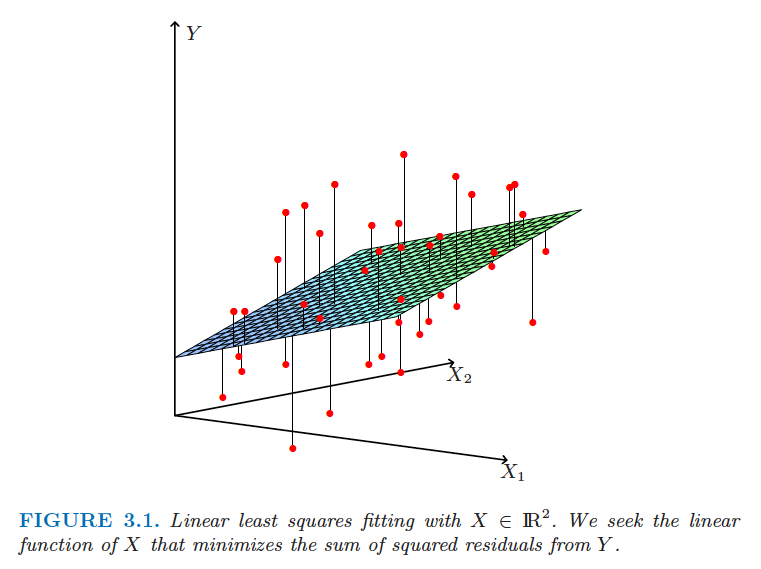
\includegraphics[width=0.6\linewidth]{geometric_int_1.png}
    
\end{figure}
\end{frame}




%-----------------------------------------------

\begin{frame}{Normal Equations}
Differentiating the RSS:

\[
\frac{\partial \text{RSS}}{\partial \beta} = -2X^T (y - X\beta), \quad
\frac{\partial^2 \text{RSS}}{\partial \beta \partial \beta^T} = 2X^T X
\]

Setting derivative to zero:

\[
X^T (y - X\beta) = 0
\]

\[
\hat{\beta} = (X^T X)^{-1} X^T y
\]
\end{frame}

%-----------------------------------------------

\begin{frame}{Geometric Interpretation}
\begin{itemize}
    \item $\hat{y} = X \hat{\beta}$ is the orthogonal projection of $y$ onto the column space of $X$.
    \item The projection matrix:
    \[
    H = X (X^T X)^{-1} X^T
    \]
    \item Called the ``hat matrix'' since $\hat{y} = Hy$.
\end{itemize}
\end{frame}

%-----------------------------------------------

\begin{frame}{Least Squares Estimation}
\begin{figure}
    \centering
    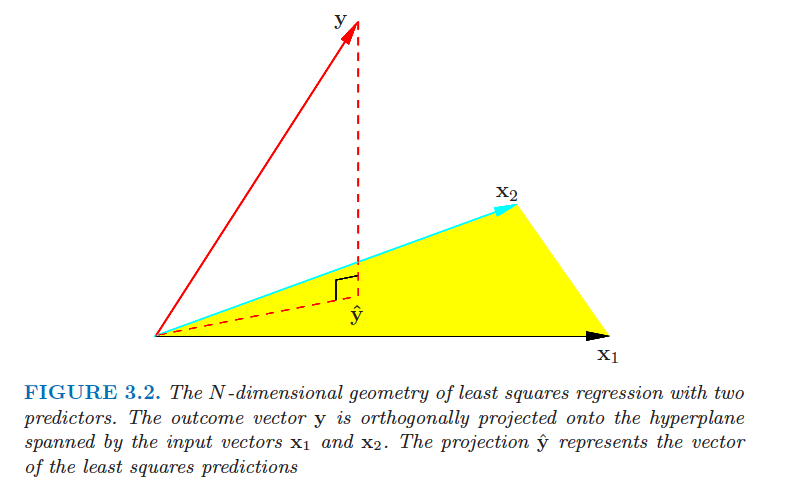
\includegraphics[width=0.6\linewidth]{geometric_int_2.png}
    
\end{figure}
\end{frame}
%-----------------------------------------------

\begin{frame}{Rank Deficiency}
If columns of $X$ are not linearly independent:
\begin{itemize}
    \item $X^T X$ is singular.
    \item $\hat{\beta}$ is not uniquely defined.
    \item Still, $\hat{y} = X\hat{\beta}$ is the projection of $y$ onto $\text{col}(X)$.
    \item Common fix: drop redundant columns or recode categorical variables.
\end{itemize}
\end{frame}

%-----------------------------------------------

\begin{frame}{Distribution of $\hat{\beta}$}
Assume the model:
\[
Y = \beta_0 + \sum_{j=1}^p X_j \beta_j + \varepsilon, \quad \varepsilon \sim N(0, \sigma^2)
\]

Then
\[
\hat{\beta} \sim N\left(\beta, (X^T X)^{-1}\sigma^2\right)
\]

and
\[
\text{Var}(\hat{\beta}) = (X^T X)^{-1}\sigma^2
\]
\end{frame}

%-----------------------------------------------

\begin{frame}{Estimating $\sigma^2$}
An unbiased estimator:
\[
\hat{\sigma}^2 = \frac{1}{N - p - 1} \sum_{i=1}^N (y_i - \hat{y}_i)^2
\]

Distributional result:
\[
(N - p - 1)\hat{\sigma}^2 \sim \sigma^2 \chi^2_{N - p - 1}
\]

Hence $\hat{\beta}$ and $\hat{\sigma}^2$ are independent.
\end{frame}

%--------------------------------------------------
\begin{frame}{Gradient Descent: Problem Setup}
We want to minimize an objective function:
\[
L(\theta) : \mathbb{R}^d \to \mathbb{R}, 
\quad \theta \in \mathbb{R}^d
\]

\begin{block}{Optimization Goal}
\[
\theta^* = \arg\min_{\theta} L(\theta)
\]
\end{block}

Key idea: iteratively move $\theta$ in the direction of the \textbf{negative gradient}, which gives the direction of steepest descent.
\end{frame}

%--------------------------------------------------
\begin{frame}{Gradient Descent: Update Rule}
At iteration $t$, update parameters:
\[
\theta^{(t+1)} = \theta^{(t)} - \eta \nabla L(\theta^{(t)})
\]

\begin{itemize}
    \item $\nabla L(\theta^{(t)})$ = gradient of the loss at current point
    \item $\eta > 0$ = learning rate (step size)
    \item Repeat until convergence (or stopping criterion)
\end{itemize}
\end{frame}

%--------------------------------------------------
\begin{frame}{Taylor Expansion Intuition}
For small step $\Delta \theta$:
\[
L(\theta + \Delta \theta) \approx L(\theta) 
+ \nabla L(\theta)^T \Delta \theta
\]

Choosing $\Delta \theta = - \eta \nabla L(\theta)$ gives:
\[
L(\theta + \Delta \theta) 
\approx L(\theta) - \eta \|\nabla L(\theta)\|^2
\]

\begin{block}{Conclusion}
Each step decreases the loss (for sufficiently small $\eta$).
\end{block}
\end{frame}

%--------------------------------------------------
\begin{frame}{Gradient Descent: Algorithm}
\begin{algorithm}[H]
\SetAlgoLined
\KwIn{Learning rate $\eta$, initial parameters $\theta^{(0)}$, maximum iterations $T$}
\For{$t = 0,1,2,\ldots,T-1$}{
    Compute gradient: $g^{(t)} \gets \nabla L(\theta^{(t)})$ \\
    Update: $\theta^{(t+1)} \gets \theta^{(t)} - \eta g^{(t)}$
}
\KwOut{Final parameters $\theta^{(T)}$}
\end{algorithm}
\end{frame}

%--------------------------------------------------
\begin{frame}{Example: Quadratic Loss}
Consider 
\[
L(\theta) = \frac{1}{2} a \theta^2, \quad a > 0
\]

Gradient:
\[
\nabla L(\theta) = a\theta
\]

Update:
\[
\theta^{(t+1)} = \theta^{(t)} - \eta a \theta^{(t)} 
= (1 - \eta a)\theta^{(t)}
\]

Convergence if $0 < \eta < \frac{2}{a}$.
\end{frame}

%--------------------------------------------------
\begin{frame}{Geometric View}
\begin{itemize}
    \item Gradient = vector of steepest ascent.
    \item Gradient descent moves in opposite direction.
    \item Learning rate controls step length:
    \begin{itemize}
        \item Too small $\;\Rightarrow\;$ slow convergence
        \item Too large $\;\Rightarrow\;$ divergence
    \end{itemize}
\end{itemize}

\begin{center}
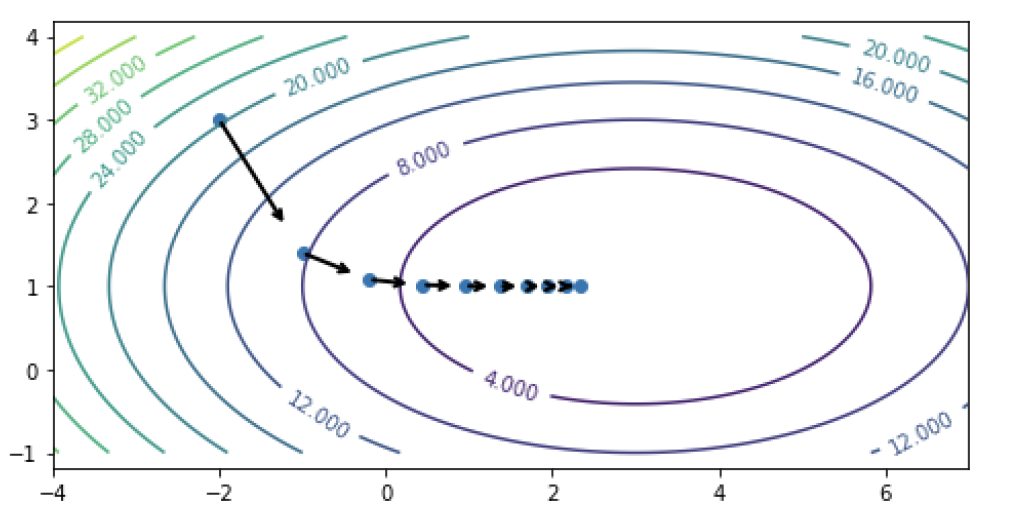
\includegraphics[width=0.6\textwidth]{sgd_method.png}
\end{center}
\end{frame}



%--------------------------------------------------
\begin{frame}{Linear Regression: Setup}
We model:
\[
\hat{y}^{(i)} = \mathbf{w}^T \mathbf{x}^{(i)} + b,
\]
where
\begin{itemize}
    \item $\mathbf{x}^{(i)} \in \mathbb{R}^p$ = input features
    \item $y^{(i)} \in \mathbb{R}$ = target
    \item $\mathbf{w} \in \mathbb{R}^p$, $b \in \mathbb{R}$ = parameters
\end{itemize}

Loss function (Mean Squared Error):
\[
L(\mathbf{w}, b) = \frac{1}{2N} \sum_{i=1}^N \big( y^{(i)} - \hat{y}^{(i)} \big)^2
= \frac{1}{2N} \sum_{i=1}^N \big( y^{(i)} - (\mathbf{w}^T \mathbf{x}^{(i)} + b) \big)^2
\]
\end{frame}

%--------------------------------------------------
\begin{frame}{Gradients for Linear Regression}
Compute gradient w.r.t. $\mathbf{w}$:
\[
\nabla_{\mathbf{w}} L(\mathbf{w}, b) 
= -\frac{1}{N} \sum_{i=1}^N \big( y^{(i)} - (\mathbf{w}^T \mathbf{x}^{(i)} + b) \big)\mathbf{x}^{(i)}
\]

Gradient w.r.t. $b$:
\[
\nabla_{b} L(\mathbf{w}, b) 
= -\frac{1}{N} \sum_{i=1}^N \big( y^{(i)} - (\mathbf{w}^T \mathbf{x}^{(i)} + b) \big)
\]
\end{frame}

%--------------------------------------------------
\begin{frame}{Gradient Descent Updates}
Gradient descent update rules:
\[
\mathbf{w} \;\;\leftarrow\;\; \mathbf{w} - \eta \nabla_{\mathbf{w}} L(\mathbf{w}, b)
\]

\[
b \;\;\leftarrow\;\; b - \eta \nabla_{b} L(\mathbf{w}, b)
\]

Explicitly:
\[
\mathbf{w} \;\;\leftarrow\;\; 
\mathbf{w} + \frac{\eta}{N} \sum_{i=1}^N \big( y^{(i)} - \mathbf{w}^T \mathbf{x}^{(i)} - b \big)\mathbf{x}^{(i)}
\]

\[
b \;\;\leftarrow\;\; 
b + \frac{\eta}{N} \sum_{i=1}^N \big( y^{(i)} - \mathbf{w}^T \mathbf{x}^{(i)} - b \big)
\]
\end{frame}

%--------------------------------------------------
\begin{frame}{Stochastic and Minibatch Versions}
\begin{itemize}
    \item \textbf{Stochastic Gradient Descent (SGD):}
    Use one sample $(x^{(i)}, y^{(i)})$ at each update:
    \[
    \mathbf{w} \;\leftarrow\; \mathbf{w} + \eta \big( y^{(i)} - \mathbf{w}^T x^{(i)} - b \big) x^{(i)}
    \]
    \[
    b \;\leftarrow\; b + \eta \big( y^{(i)} - \mathbf{w}^T x^{(i)} - b \big)
    \]
    \item \textbf{Minibatch SGD:}
    Average gradients over a minibatch $\mathcal{B}_t$:
    \[
    \mathbf{w} \;\leftarrow\; \mathbf{w} + \frac{\eta}{|\mathcal{B}_t|} 
    \sum_{i \in \mathcal{B}_t} \big( y^{(i)} - \mathbf{w}^T x^{(i)} - b \big)x^{(i)}
    \]
    \[
    b \;\leftarrow\; b + \frac{\eta}{|\mathcal{B}_t|} 
    \sum_{i \in \mathcal{B}_t} \big( y^{(i)} - \mathbf{w}^T x^{(i)} - b \big)
    \]
\end{itemize}
\end{frame}

%--------------------------------------------------
\begin{frame}{The Goal of Linear Regression}
\begin{itemize}
    \item We have inputs $x^{(i)}$ and outputs $y^{(i)}$.
    \item We want to draw a line (or plane) that best predicts $y$ from $x$.
    \item The line looks like:
    \[
    \hat{y} = w^T x + b
    \]
    where $w$ are the slopes (weights) and $b$ is the intercept.
\end{itemize}
\end{frame}

%--------------------------------------------------
\begin{frame}{The Error (Loss Function)}
\begin{itemize}
    \item The line is never perfect.
    \item Each point has an error:
    \[
    \text{error}^{(i)} = y^{(i)} - (w^T x^{(i)} + b)
    \]
    \item We square the errors and add them up to measure “how bad” the line is.
    \item This is called the \textbf{loss function}.
\end{itemize}
\end{frame}

%--------------------------------------------------
\begin{frame}{Idea of Gradient Descent}
\begin{itemize}
    \item Imagine you are standing on a hill:
    \begin{itemize}
        \item Height = loss (how bad the line is).
        \item Position = current guess of $w$ and $b$.
        \item Slope = direction of steepest increase.
    \end{itemize}
    \item To minimize the loss:
    \begin{block}{Rule}
    Take a small step downhill, then repeat, until you reach the bottom.
    \end{block}
\end{itemize}
\end{frame}

%--------------------------------------------------
\begin{frame}{How the Updates Work}
\begin{itemize}
    \item We calculate the slope (gradient) of the loss with respect to $w$ and $b$.
    \item These slopes tell us how to adjust $w$ and $b$.
    \item Update rule:
    \[
    w \leftarrow w - \eta \cdot \text{slope of } w
    \]
    \[
    b \leftarrow b - \eta \cdot \text{slope of } b
    \]
    \item $\eta$ is the \textbf{learning rate} = size of the step.
\end{itemize}
\end{frame}

%--------------------------------------------------
\begin{frame}{Different Versions of Gradient Descent}
\begin{itemize}
    \item \textbf{Batch Gradient Descent:} use all data at once (slow but exact).
    \item \textbf{Stochastic Gradient Descent (SGD):} update using one random point at a time (fast but noisy).
    \item \textbf{Minibatch Gradient Descent:} update using a small random batch (balance of speed and accuracy).
\end{itemize}

\begin{block}{Key Idea}
No matter which version we use, repeating updates makes the line get closer to the best fit.
\end{block}
\end{frame}


%--------------------------------------------------
\begin{frame}{Linear Regression and the Normal Distribution}
\begin{itemize}
    \item So far, squared loss was motivated as a convenient way to measure error.
    \item We can also justify it probabilistically using the \textbf{normal distribution}.
    \item Linear regression was developed in the 19th century (Legendre, Gauss).
    \item Gauss also introduced the normal distribution, showing a deep connection.
\end{itemize}
\end{frame}

%--------------------------------------------------
\begin{frame}{The Normal Distribution}
A normal (Gaussian) distribution with mean $\mu$ and variance $\sigma^2$ is:
\[
p(x) = \frac{1}{\sqrt{2\pi\sigma^2}}
\exp\left( - \frac{1}{2\sigma^2} (x - \mu)^2 \right).
\]
\end{frame}

%--------------------------------------------------
\begin{frame}{From Regression with Noise to a Distribution}
We start with the regression model:
\[
y = \mathbf{w}^\top \mathbf{x} + b + \varepsilon, 
\quad \varepsilon \sim \mathcal{N}(0, \sigma^2).
\]

\begin{itemize}
    \item The noise $\varepsilon$ is Gaussian with mean $0$ and variance $\sigma^2$.
    \item This implies:
    \[
    y \sim \mathcal{N}(\mathbf{w}^\top \mathbf{x} + b, \, \sigma^2).
    \]
    \item Recall: if $Y \sim \mathcal{N}(\mu, \sigma^2)$, then its density is:
    \[
    p(y) = \frac{1}{\sqrt{2\pi\sigma^2}} 
    \exp\left(-\frac{1}{2\sigma^2}(y - \mu)^2\right).
    \]
    \item Substituting $\mu = \mathbf{w}^\top \mathbf{x} + b$, we get:
    \[
    P(y \mid \mathbf{x}) 
    = \frac{1}{\sqrt{2\pi\sigma^2}}
    \exp\left( -\frac{1}{2\sigma^2}(y - \mathbf{w}^\top \mathbf{x} - b)^2 \right).
    \]
\end{itemize}
\end{frame}


%--------------------------------------------------
\begin{frame}{Likelihood Function}
For independent observations $\{(x^{(i)}, y^{(i)})\}_{i=1}^n$:

\[
P(\mathbf{y} \mid X) = \prod_{i=1}^n P(y^{(i)} \mid x^{(i)})
= \prod_{i=1}^n \frac{1}{\sqrt{2\pi\sigma^2}}
\exp\left( - \frac{1}{2\sigma^2} (y^{(i)} - \mathbf{w}^\top x^{(i)} - b)^2 \right).
\]

\begin{block}{Principle of Maximum Likelihood}
The best parameters $\mathbf{w}, b$ are those that maximize this likelihood.
\end{block}
\end{frame}

%--------------------------------------------------
\begin{frame}{Negative Log-Likelihood}
It is easier to maximize the log-likelihood:
\[
\log P(\mathbf{y} \mid X) 
= - \frac{n}{2} \log(2\pi\sigma^2) 
- \frac{1}{2\sigma^2} \sum_{i=1}^n \big(y^{(i)} - \mathbf{w}^\top x^{(i)} - b \big)^2.
\]

Equivalently, minimize the \textbf{negative log-likelihood}:
\[
- \log P(\mathbf{y} \mid X) 
= \sum_{i=1}^n \frac{1}{2\sigma^2} \big(y^{(i)} - \mathbf{w}^\top x^{(i)} - b \big)^2 
+ \frac{n}{2}\log(2\pi\sigma^2).
\]
\end{frame}

%--------------------------------------------------
\begin{frame}{Connection to Squared Loss}
\begin{itemize}
    \item The second term does not depend on $\mathbf{w}, b$.
    \item Minimizing the negative log-likelihood is equivalent to minimizing:
    \[
    \sum_{i=1}^n \big(y^{(i)} - \mathbf{w}^\top x^{(i)} - b \big)^2
    \]
    \item \textbf{Conclusion:} Squared error loss arises naturally from the assumption of Gaussian noise.
\end{itemize}
\end{frame}










% %--------------------------------------------------
% \begin{frame}{Stochastic Gradient Descent (SGD)}
% We want to minimize the empirical risk:
% \[
% L(\mathbf{w}, b) = \frac{1}{N} \sum_{i=1}^N \ell^{(i)}(\mathbf{w}, b),
% \]
% where $\ell^{(i)}$ is the loss for the $i$-th example.

% \begin{itemize}
%     \item \textbf{Full-batch gradient descent:}
%     \[
%     (\mathbf{w}, b) \leftarrow (\mathbf{w}, b) - \eta \nabla L(\mathbf{w}, b)
%     \]
%     requires computing gradient over all $N$ examples.
%     \item \textbf{Stochastic gradient descent (SGD):}
%     \[
%     (\mathbf{w}, b) \leftarrow (\mathbf{w}, b) - \eta \nabla \ell^{(i)}(\mathbf{w}, b)
%     \]
%     uses a single random example per update.
% \end{itemize}
% \end{frame}

% %--------------------------------------------------
% \begin{frame}{Drawbacks of Pure SGD}
% \begin{itemize}
%     \item Each update is noisy $\;\Rightarrow\;$ high variance in convergence.
%     \item Works well for large datasets, but may converge slowly.
%     \item Some operations (e.g., batch normalization) require more than one sample.
% \end{itemize}

% \[
% \text{Trade-off: Efficiency vs. Variance of updates.}
% \]
% \end{frame}

% %--------------------------------------------------
% \begin{frame}{Minibatch Stochastic Gradient Descent}
% Intermediate strategy: update using a small batch of size $|\mathcal{B}_t|$.

% At iteration $t$, sample a minibatch $\mathcal{B}_t \subseteq \{1,\ldots,N\}$.

% \[
% (\mathbf{w}, b) \;\;\leftarrow\;\; (\mathbf{w}, b) 
% - \frac{\eta}{|\mathcal{B}_t|} \sum_{i \in \mathcal{B}_t} 
% \nabla \ell^{(i)}(\mathbf{w}, b)
% \]

% \begin{itemize}
%     \item $|\mathcal{B}_t| = 1 \;\Rightarrow\;$ SGD
%     \item $|\mathcal{B}_t| = N \;\Rightarrow\;$ batch gradient descent
%     \item Typically: $32 \leq |\mathcal{B}_t| \leq 256$
% \end{itemize}
% \end{frame}

% %--------------------------------------------------
% \begin{frame}{Example: Squared Loss}
% For linear regression with loss
% \[
% \ell^{(i)}(\mathbf{w}, b) = \frac{1}{2}\big( y^{(i)} - \mathbf{w}^T \mathbf{x}^{(i)} - b \big)^2,
% \]

% the minibatch update is:
% \[
% \mathbf{w} \leftarrow \mathbf{w} - \frac{\eta}{|\mathcal{B}_t|} 
% \sum_{i \in \mathcal{B}_t} \big( \mathbf{w}^T \mathbf{x}^{(i)} + b - y^{(i)} \big)\mathbf{x}^{(i)},
% \]

% \[
% b \leftarrow b - \frac{\eta}{|\mathcal{B}_t|} 
% \sum_{i \in \mathcal{B}_t} \big( \mathbf{w}^T \mathbf{x}^{(i)} + b - y^{(i)} \big).
% \]
% \end{frame}


% %--------------------------------------------------
% \begin{frame}{Geometric Intuition for SGD}
% \begin{itemize}
%     \item Gradient descent moves parameters $(\mathbf{w}, b)$
%     in the direction of the negative gradient of the loss.
%     \item Full-batch gradient descent:
%     \[
%     \Delta \theta = - \eta \nabla L(\theta), 
%     \quad \theta = (\mathbf{w}, b)
%     \]
%     always points toward the global minimum.
%     \item SGD:
%     \[
%     \Delta \theta = - \eta \nabla \ell^{(i)}(\theta)
%     \]
%     uses one sample $\Rightarrow$ update is \emph{noisy}.
% \end{itemize}

% \vspace{0.3cm}
% \begin{block}{Key Idea}
% SGD takes \textbf{zig-zagging steps} that approximate the
% true gradient direction. Over time, the noise averages out
% and the trajectory approaches the minimum.
% \end{block}

% \end{frame}
\end{document}
